\section{Question 3: Fixed-split cross-GPU substitution}
\label{sec:r1q3}
\subsection{Model and two versions of the route rule}
A job has native model $n_j$, actual model $m_j$, duration $p_j$, workers $W_j$, and per-worker requests $(g_j,c_j)$. For the sole assumed foreign edge A10$\to$A100-SXM4-80GB, $p'_j=\sigma p_j$; compatibility and $\sigma$ are scenario assumptions, not measured hardware facts. All workers start together on physical nodes, with no migration or preemption, and every start passes the same CPU/GPU slot check.

V1/S1--S5 are the historical fixed-split sensitivity runs: M0 is model isolated, and R0 (called S0 in the historical tables) reserves 60 of 432 A100 nodes for a 10\% SHA-256-selected A10 subset. V2 C0--C4 are the complete merged-runtime cases; GS1 uses ratio placement, while other pools use FF-id. The implemented V2 substitution rule is \emph{R-shape}; only Candidate B (online completion-cost routing) remains deferred. R-shape keeps only hash-selected jobs whose CPU/GPU shape fits the donor ratio, yielding 10,604 routed and 605 shape-rejected A10 jobs. It is a fixed physical counterfactual, not a claim that a dynamic policy has been implemented.

\begin{table}[H]\centering\caption{SPT-HOL V2 substitution evidence from persisted full-cluster results. Native harm is the number of native A100 jobs with positive additional waiting relative to M0; the final column is the principal harmed A10 group relative to M0.}\label{tab:r1q3main}\begin{tabular}{lrrrrrr}
\toprule
Scenario & $\sigma$ & A10 wait (h) & A10 JCT (h) & All JCT (h) & $90$d done & Native harm / A10 harmed\\
\midrule
M0 & -- &32.906&132.676&93.353&217,570&0 / 0\\
R0 &1&20.534&120.303&87.209&217,814&0 / 49,772\\
R0 &2&25.106&134.810&94.412&217,521&0 / 56,422\\
R-shape &1&24.359&124.128&89.108&217,801&0 / 46,803\\
R-shape &2&24.359&129.671&91.860&217,613&0 / 55,465\\
\bottomrule
\end{tabular}\end{table}

For FCFS, R0 $\sigma=1$ gives A10 mean wait 587.875 h and all-job mean JCT 368.910 h; R-shape gives 656.356 h and 402.914 h. At $\sigma=2$, FCFS R0 has A10 mean JCT 831.456 h, whereas R-shape has 761.668 h. Thus the largest-JCT comparison is favorable to R-shape at both tested speeds for the displayed policy, while R0 is better for SPT-HOL at $\sigma=1$ (A10 JCT 120.303 versus 124.128 h). These are two measured points, not an upper bound over $[1,2]$, an unknown-speed guarantee, or a unique $\sigma^*$.

\subsection{What the trade-off means}
For SPT-HOL, R0 is the more aggressive 10\% split; R-shape rejects 605 high-CPU/GPU jobs and changes the selected load. At $\sigma=1$, R0 reduces A10 wait relative to M0, while R-shape has a smaller A10 benefit but lower paired positive completion-delay mass (16,051.659 job-hours versus R0's 68,183.183 job-hours). At $\sigma=2$, common routed-job ordering is unchanged because all durations in one foreign queue are multiplied by the same $\sigma$; re-simulation is still required because completion/release interactions change. R-shape's A10 wait is unchanged at 24.359 h between the two tested speeds, but A10 JCT rises 5.542 h and 90-day completions fall by 188.

The A100 physical allocation comparison uses one full-pool denominator of 3,456 GPUs and sums native plus foreign occupancy. For SPT-HOL, R0 $\sigma=1$ is 0.7224 (native 2,976-GPU partition 0.6276 plus foreign 480-GPU partition 0.0948); R-shape is 0.6899 at $\sigma=1$ (0.7288 native plus 0.4492 foreign) and 0.7148 at $\sigma=2$ (0.7288 plus 0.6284). A larger partition rate is not called a utilization gain by shrinking the native denominator.

\begin{figure}[H]\centering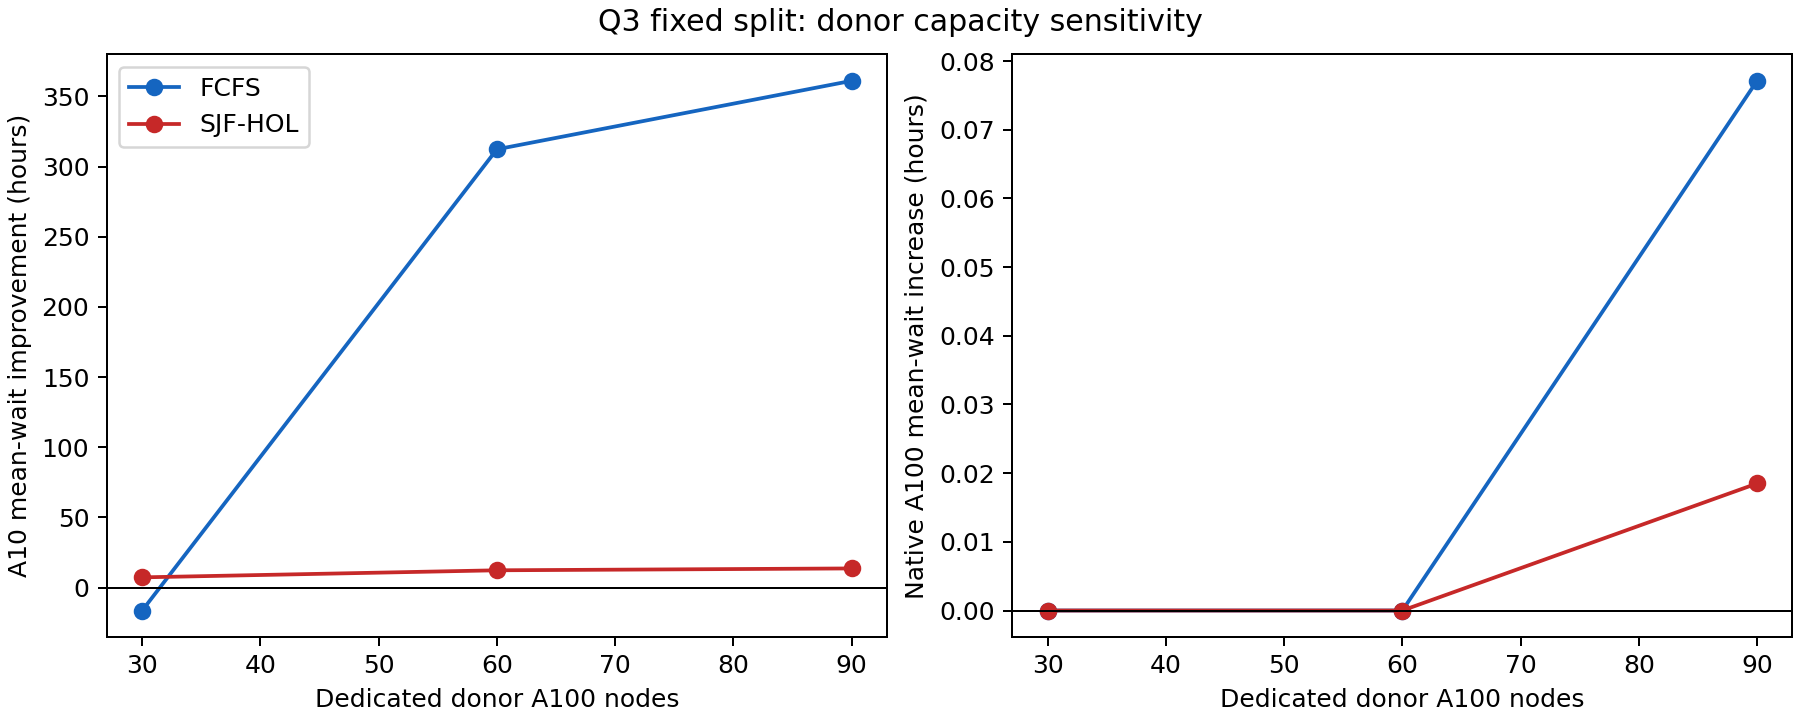
\includegraphics[width=0.86\linewidth]{figures/q3_donor_capacity_wait_tradeoff.png}\caption{V1/S1--S5 donor-capacity sensitivity. The left panel is A10 mean-wait change; the right panel is native A100 mean-wait change, with separate scales.}\label{fig:r1q3tradeoff}\end{figure}

The historical sensitivity retains its negative cases: at 60 donors, 20\% routing raises FCFS A10 mean wait to 1,010.136 h and its maximum to 5,445.367 h; 30 donors at 10\% gives 916.407 h, worse than M0. For the 90-donor case, SPT-HOL native A100 has 2,150 positive-delay jobs, mean additional wait 0.018492 h over all 80,877 native jobs, and harmed-subgroup mean 0.695606 h. These finite paired results expose the management choice between A10 relief, native harm, tail, and completion count.

A financial extension is optional rather than a second experiment. If a tenant values completion time at $v$ per hour and pays $P$, voluntary substitution requires payment reduction at least $v$ times the completion-time increase. No price, participation rate, revenue, or profitability is inferred here. The online Candidate B rule is recorded as future work, and no new 480-job batch policy or borrowed threshold is introduced.
